\section{Spezifikation von Einflussfaktoren}
\label{influencingfactors}

Aus denen im Abschnitt \ref{environment} und \ref{futuretrends} dargestellten Umweltfaktoren sowie Zukunftstrends lassen sich nun im Folgenden relevante Einflussfaktoren für den Einsatz von Cloud Computing für die fiktive Skola GmbH herausarbeiten.

\subsection{Ermittlung der Einflussfaktoren}

Die Erarbeitung der Einflussfaktoren erfolgte aus einer umfassenden Literaturrecherche, sowie Experteninterviews mit Vertretern aus der Bildungsbranche. Innerhalb dieser Literaturrecherche wurde gezielt nach solchen Faktoren gesucht, die zu einem Einsatz von Cloud Computing auf Unternehmensebene führten, aber auch nach solchen, die davon abhielten. Dazu gehörten u.a. Ängste und Nachteile der Technologie. Anschließend wurden die gefundenen Faktoren gruppiert und (positive) Einflussfaktoren definiert. Diese finden sich in der Tabelle \ref{tab:factors1}.

Die genauen Beschreibungen aller Einflussfaktoren ist nicht Teil dieser Arbeit. Die große Anzahl an gefundenen Einflussfaktoren stört bei der Erstellung von zukunftstauglichen Szenarien. Nachfolgend sollen diese mittels einem Faktorenportfolio und einer Einflussmatrix weiter eingegrenzt werden.

\FloatBarrier
\begin{table}[!htb]
	\caption{Übersicht der Einflussfaktor im Suchfeld \textit{Cloud Computing}}
	\begin{center}
		\resizebox{\linewidth}{!}{
			\begin{tabular}{c c c }
				\hline
				\textbf{Nummer} & \textbf{Einflussfaktor} & \textbf{Referenz} \\
				\hline
				1 & Ausfallsicherheit & Gebauer et al. \cite{gebauer }, Schweizer \cite{schweizer} \\
				2 & Informationssicherheit & Gebauer et al. \cite{gebauer}, Meinel et al. \cite{meinel}, \\
				&& Almajalid \cite{almajalid}, Chandra et al. \cite{chandra}, \\
				&& Schweizer \cite{schweizer},  Renz \cite{renz} \\
				3 & Störungssicherheit im Netzwerk & Gebauer et al. \cite{gebauer} \\
				4 & Skalierbarkeit & Gebauer et al. \cite{gebauer}, Stieninger \cite{stieninger}, \\
				&& Almajalid \cite{almajalid}, Renz \cite{renz} \\
				5 & Flexible Finanzierungsmodelle & Gebauer et al. \cite{gebauer}, Almajalid \cite{almajalid} \\
				6 & Zuverlässige und schnelle & Gebauer et al. \cite{gebauer}, Stieninger \cite{stieninger}, \\
				& Datenübertragung & Almajalid \cite{almajalid} \\
				7 & Datenintegrität & Gebauer et al. \cite{gebauer} \\
				8 & Unabhängigkeit vom Anbieter & Gebauer et al. \cite{gebauer}, Grella et al. \cite{grella} \\
				9 & Unabhängigkeit von anderen Nutzern & Gebauer et al. \cite{gebauer}, Grella et al. \cite{grella} \\
				10 & Kontrollmöglichkeiten (on Demand) & Gebauer et al. \cite{gebauer}, Stieninger \cite{stieninger}, \\
				&& Alabbadi \cite{alabbadi} \\
				11 & Reliabilität \& Transparenz & Gebauer et al. \cite{gebauer} \\
				12 & Einhaltung rechtlicher Standards & Gebauer et al. \cite{gebauer} \\
				13 & Orts - \& Zeitunabhängigkeit & Stieninger \cite{stieninger}, Meinel et al. \cite{meinel} \cite{meinel2}, \\
				&& Almajalid \cite{almajalid} \\
				14 & Optimierte Ressourcenauslastung & Stieninger \cite{stieninger}, Almajalid \cite{almajalid}, \\
				&& Alabbadi \cite{alabbadi}, Renz \cite{renz} \\
				15 & Energieeffizienz & Stieninger \cite{stieninger} \\
				16 & Modernes Image & Stieninger \cite{stieninger} \\
				17 & Vernetzung von organisatorischen & Stieninger \cite{stieninger}, Meinel et al. \cite{meinel}, \\
				& und prozessualen Strukturen & Chandra et al. \cite{chandra}, Krcmar et al. \cite{krcmar} \\
				18 & Benutzerfreundlichkeit & Stieninger \cite{stieninger}, Almajalid \cite{almajalid} \\
				\hline
			\end{tabular}
		}
		\label{tab:factors1}
	\end{center}
\end{table}
\FloatBarrier

\subsection{Faktorenportfolio}

\begin{figure}
	\centering
	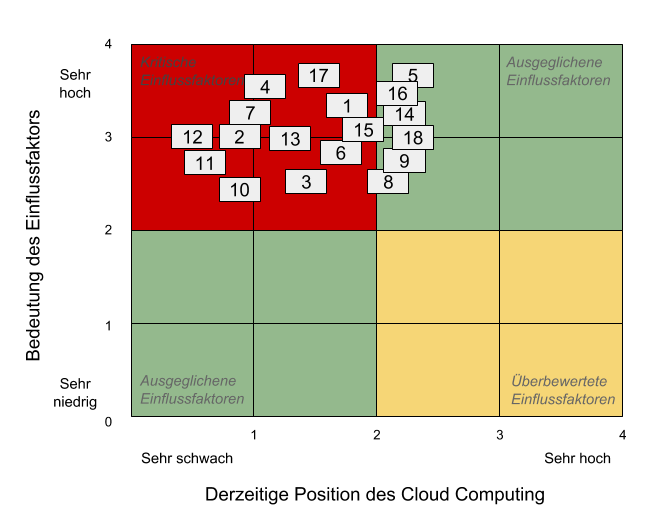
\includegraphics[width=\linewidth]{images/portfolio}
	\caption[Caption for parameters]{Faktorenportfolio}
	\label{fig:portfolio}
\end{figure}

\subsection{Einflussmatrix}

\begin{figure}
	\centering
	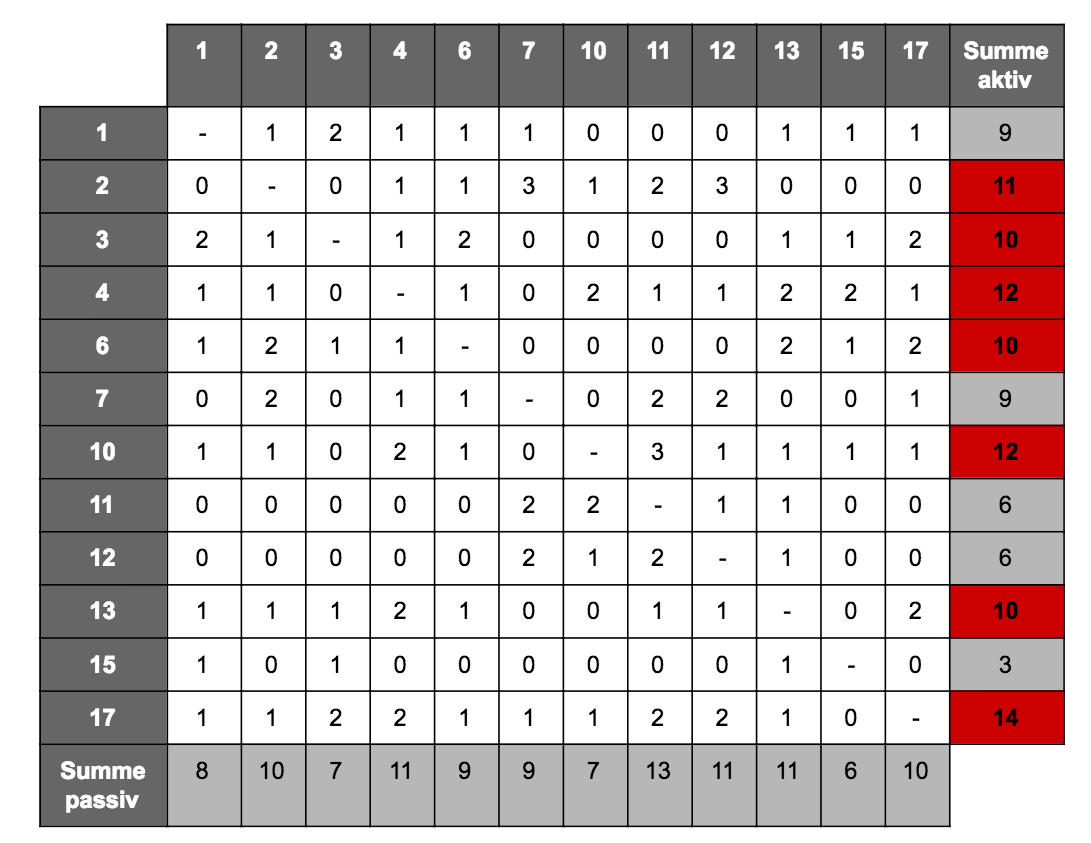
\includegraphics[width=\linewidth]{images/matrix}
	\caption[Caption for parameters]{Einflussmatrix}
	\label{fig:matrix}
\end{figure}

\subsection{Beschreibung der Schlüsselfaktoren}